% --------------------------------------------------------------

\documentclass[spanish, letterpaper,12]{article}

\usepackage[activeacute]{babel}
\usepackage[utf8x]{inputenc}
\usepackage[T1]{fontenc}
\spanishdecimal{.}

\usepackage{amsmath,amsthm,amssymb}
\usepackage[margin=1in]{geometry} 
\usepackage{graphicx}
\usepackage{hyperref}
\usepackage[numbers]{natbib}
\usepackage{enumitem} % para reducir el espacio [noitemsep,nolistsep]
\usepackage{verbatim}

\usepackage{mathtools}
\usepackage{booktabs} % para las tablas \toprule \bo

\DeclareGraphicsExtensions{.pdf,.png,.jpg}
\graphicspath{{./fig/}}


\usepackage{fancyhdr}
\renewcommand{\headrulewidth}{0pt}
\fancyhead[C]{
\includegraphics[width=3cm]{upa.jpg}}
\fancyhead[R]{}


\newcommand{\N}{\mathbb{N}}
\newcommand{\Z}{\mathbb{Z}}
 
\newenvironment{theorem}[2][Teorema]{\begin{trivlist}
\item[\hskip \labelsep {\bfseries #1}\hskip \labelsep {\bfseries #2.}]}{\end{trivlist}}
\newenvironment{lemma}[2][Lemma]{\begin{trivlist}
\item[\hskip \labelsep {\bfseries #1}\hskip \labelsep {\bfseries #2.}]}{\end{trivlist}}
\newenvironment{exercise}[2][Ejercicio]{\begin{trivlist}
\item[\hskip \labelsep {\bfseries #1}\hskip \labelsep {\bfseries #2.}]}{\end{trivlist}}
\newenvironment{problem}[2][Problema]{\begin{trivlist}
\item[\hskip \labelsep {\bfseries #1}\hskip \labelsep {\bfseries #2.}]}{\end{trivlist}}
\newenvironment{question}[2][Pregunta]{\begin{trivlist}
\item[\hskip \labelsep {\bfseries #1}\hskip \labelsep {\bfseries #2.}]}{\end{trivlist}}
\newenvironment{corollary}[2][Corollary]{\begin{trivlist}
\item[\hskip \labelsep {\bfseries #1}\hskip \labelsep {\bfseries #2.}]}{\end{trivlist}}



\begin{document}
 
% --------------------------------------------------------------
%                         Start here
% --------------------------------------------------------------
\title{Serie de Ejercicios}
\author{Profesor: Dr. Isaías Moreno Cruz\\
  Ingeniería en Energía Fototérmica (2023)\\
Universidad Politécnica de Aguascalientes (UPA)}
\date{13 de octubre de 2023}

\maketitle

\begin{itemize}[leftmargin=*, noitemsep]
\item \textbf{Fecha de encargo:} viernes 13 de octubre
\item \textbf{Fecha de entrega:} lunes 23 de octubre
\end{itemize}
% You can use theorem, exercise, problem, or question here.
% --------------------------------------------------------------
\thispagestyle{fancy}

\begin{problem}{1}

  La Fig.~\ref{fig:dia2014} muestra el comportamiento de la irradiancia global $G$, directa $G_{b}$ y difusa $G_{d}$ el día 5 de diciembre de 2014 en Temixco, Morelos. El archivo \verb|dia2014.csv| contiene la información de la irradiancia $G$, $G_{b}$ y $G_{d}$. Calcular la irradiancia directa a partir de la irradiancia global y la difusa, además de calcular el error RMSE de la radiación directa calculada contra la medida por el pirheliómetro.

\begin{figure}[ht]
  \centering
  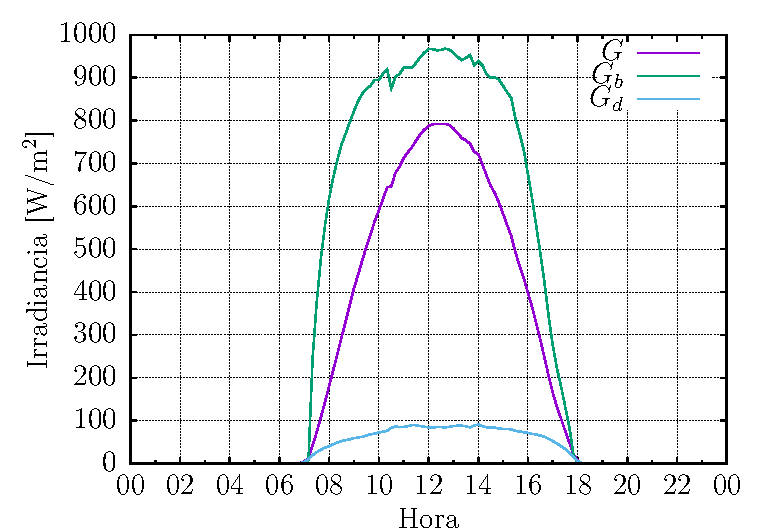
\includegraphics[width=0.8\textwidth]{dia2014}
  \caption{\label{fig:dia2014} Comportamiento de la irradiancia el día 5 de dociembre de 2014, en Temixco Morelos.}
\end{figure}

\end{problem}

\begin{problem}{2}

  El archivo \verb|data_2014.csv| contiene la irradiancia global $G$, directa $G_{b}$ y difusa $G_{d}$ del año 2014, en Temixco, Morelos. Calcula la irradiancia promedio diaria mensual $\bar{H}$ en [MJ/m$^{2}$] del año 2014, para la irradiancia global, directa y difusa. Mostrar gráficamente e indicar una tabla.

\end{problem}

\begin{problem}{3}
  Considerando el archivo \verb|data_2014.csv| de irradiacia del Temixco, Morelos. Calcula el índice de claridad diario $K_{T}$ para los día del mes de enero.
\end{problem}

\begin{problem}{4}
  Calcula la insolación promedio $\bar{H}_{I}$ para un colector inclinado a la latitud, en Temixco, para cada mes del año 2014.Gráfica tus resultados.
\end{problem}


\section*{Formulario}
\label{sec:Formulario}
% ----------------------------------------------------------------------

\subsection{Error RMSE}
\label{subsec:error}

La comparación estadística de estimación o predicción de modelos ($P_i$; $i=1,2,\ldots,n$) pensando que es una estimación de las observaciones ($O_i$;$i=1,2,\ldots,n$) continua ocurriendo en la practica de
La mayoria de los modelos básicos de evaluación del comportamiento climatico y en ciencias ambientales.

Los errores de predicción de modelos individuales son usualmente definidos como:

\begin{equation}
    \label{eq:error}
    e_i = P_i - O_i
  \end{equation}
  donde $P_{i}$ son las predicciones de modelos y $O_{i}$ son las observaciones.

  El error \textbf{RMSE}, por sus siglas en ingles de /root mean square error/ ha sido usado como una métrica estadística estándar para el comportamiento de modelos en meteorologia, calidad del aire, e investigaciones relacionadas con el clima. El RMSE se define como:

  \begin{equation}
    \label{eq:rmse}
    RMSE = \sqrt{ \dfrac{1}{n} \sum_{i=1}^n e_i^2 }
  \end{equation}

  El RMSE es más apropiado para representar modelos donde la distribución de error tiene un comportamiento Gausiano.

\end{document}





